% ------------------------------------------------------------------------
\subsection{CGAL Polyhedron}

CGAL Polyhedron (\cgalpoly) is realized as a container class 
that manages geometry items such as vertices, halfedges, and 
facets with their incidences.  \cgalpoly\ has chosen the 
halfedge data structure as the underlying connectivity 
structure. In the halfedge data structure, a halfedge is 
associated with a facet and stores the adjacency pointers 
to it previous, next and opposite halfedge (\figurename\ \ref{fig:halfedge}). 
The details of the halfedge data structure and the \cgalpoly\ based 
on it are described in~\cite{k-ugpdd-99}.

\begin{figure}[h]
    \centering{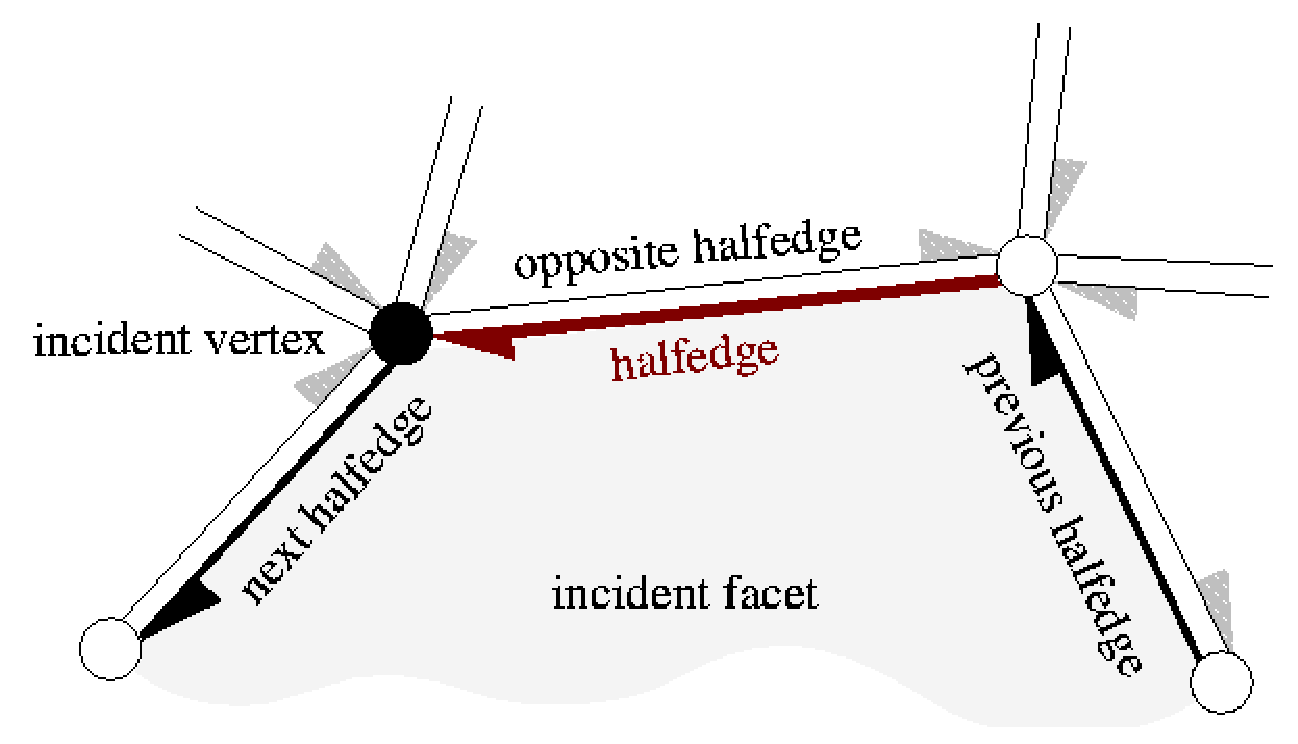
\includegraphics[width=7.0cm]{figs/halfedge}}
    \caption{One halfedge and its incident primitives. The next
      halfedge, the opposite halfedge, and the incident vertex are
      mandatory, the remaining elements are optional.
    }
    \label{fig:halfedge}
\end{figure}

What are the potential obstacles in using CGAL and \cgalpoly?
\begin{enumerate}
  \item
    Is it fast enough? Yes. \cgal, coming from the field of Computational
    Geometry, might have a reputation of using slow exact arithmetic
    to be on the safe side, but nonetheless, we know where to apply
    the right techniques of exact arithmetic to gain robustness and
    yet not to loose efficiency. In addition, \cgal\ uses
    \emph{generic programming\/} and \emph{compile-time
    polymorphism\/} to realize flexibility without affecting optimal
    runtime.
  \item
    Is it small enough? Yes. \CodeFmt{CGAL::Polyhedron \_3} can be
    tailored to store exactly the required incidences and other
    required data, not more and not less.
  \item
    Is it flexible enough? Yes, certainly within its design
    space of oriented 2-manifold meshes with boundary that was
    sufficient for the range of applications illustrated with our
    example programs. 
  \item
    Is it easy enough to use? Yes. The full tutorial with its example
    programs are exactly the starting point for using \cgalpoly. The
    example programs are short and easy to understand. There is
    certainly a learning curve for mastering \CC\ to the level
    of using templates, but it has to be emphasized that
    using templates is far easier then developing templated code.
  \item
    What is the license, can I use it? Yes, we hope so. \cgal\ since
    release 3.0 and our tutorial programs have open source
    licenses. Other options are available.
\end{enumerate}

% ------------------------------------------------------------------------
\subsection{Subdivision Surfaces}

A subdivision algorithm recursively 
applies \emph{refinement} and \emph{geometry smoothing} 
on the control mesh (\figurename\ \ref{fig:sqrt3},  
\ref{fig:quad-triangle}), 
and approximates the limit surface of the control mesh.  Several
refinement schemes in practice are illustrated in
\figurename\ \ref{fig:RefSchemes}. The stencils of the
geometry smoothing are depending on the refinement schemes, 
i.e.\ the reparameterizations. A stencil defines a control
submesh that is associated with normalized weights of the 
nodes. \figurename\ \ref{fig:RefMap} 
demonstrates the stencils of the PQQ scheme  
in Catmull-Clark subdivision \cite{cc} and DQQ scheme in Doo-Sabin
subdivision \cite{ds}. We also demonstrate Loop \cite{loop}, 
$\sqrt{3}$ \cite{sqrt3} and Quad-Triangle \cite{qts} subdivisions 
in this tutorial. For further details about subdivisions, readers
should refer to \cite{Warren:subdivision} and \cite{Sub:course:2000}.
   
\begin{figure}[tb]
  \centering
  \psfrag{PQQ}[]{\scriptsize PQQ} 
  \psfrag{PTQ}[]{\scriptsize PTQ}
  \psfrag{DQQ}[]{\scriptsize DQQ} 
  \psfrag{Sqrt3}[]{\scriptsize $\sqrt{3}$} 
  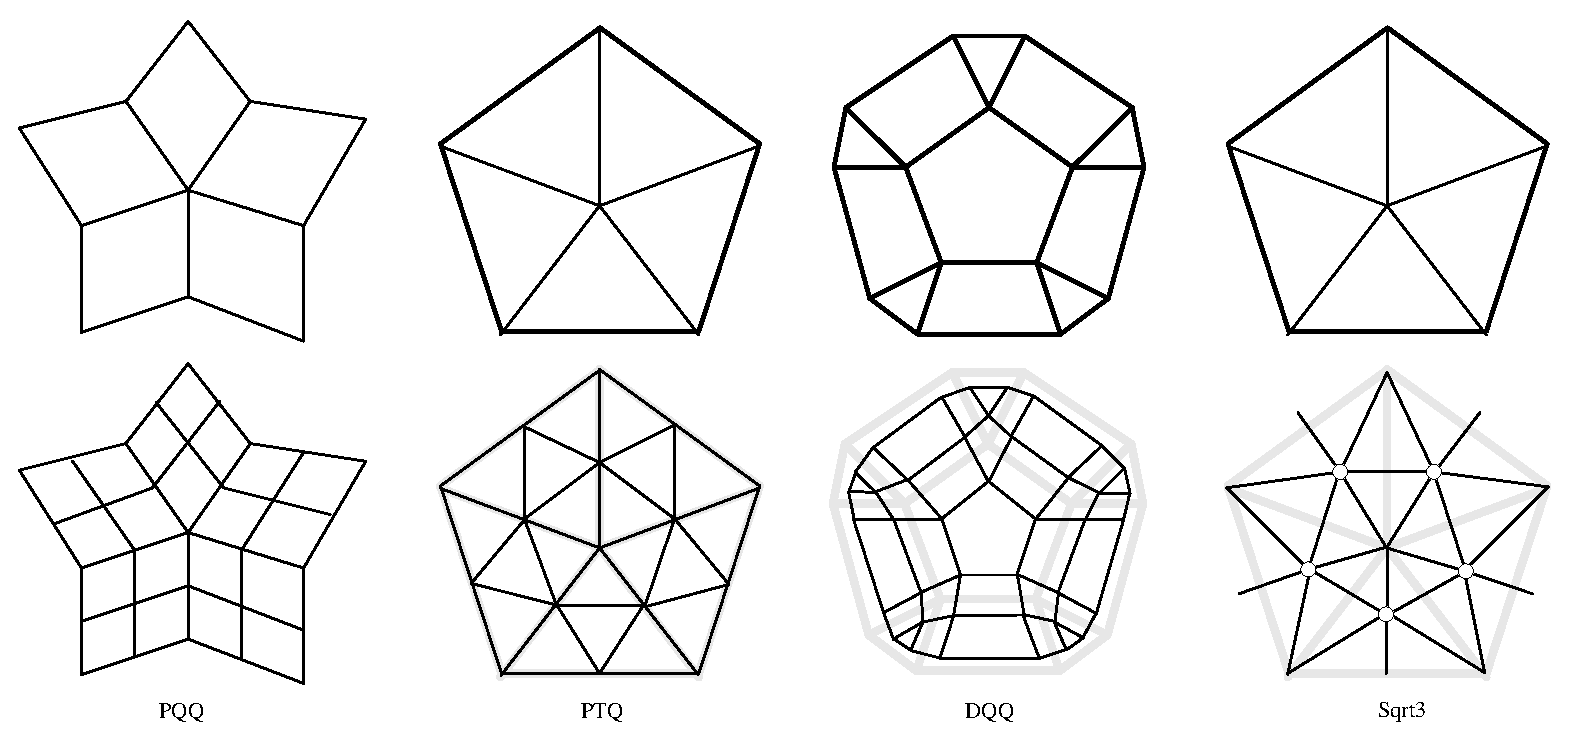
\epsfig{file=figs/RefSchemes.eps, width=12cm}
  \caption{Examples of refinement schemes: 
    primal quadrilateral quadrisection (PQQ),
    primal triangle quadrisection (PTQ),
    dual quadrilateral quadrisection (DQQ) and
    $\sqrt{3}$ triangulation. The control meshes are shown
    in the first row.}
  \label{fig:RefSchemes}
\end{figure}

\begin{figure}[h]
  \centering
  \psfrag{A}[]{(a)}
  \psfrag{B}[]{(b)}
  \psfrag{C}[]{(c)}
  \psfrag{D}[]{(d)}
  \epsfig{file=figs/RefMap.eps, width=12cm}
  \caption{The stencil ({\itshape top blue}) and its 
           vertex ({\itshape bottom red}) in 
           Catmull-Clark subdivision (a-c)
           and Doo-Sabin subdivision (d). Catmull-Clark
           subdivision has three stencils: facet-stencil (a), 
           edge-stencil (b) and vertex-stencil (c). 
           Doo-Sabin subdivision has only corner-stencil (d).
           The stencil weights are not shown.}
  \label{fig:RefMap}
\end{figure}


% ------------------------------------------------------------------------
%% \section{FAQs}

%% We compile a list of questions concerned about the tutorial and the
%% accompanying source codes and libraray.   
 
%% \begin{itemize}

%% \item Why should I read this tutorial? I am not interested in subdivisions. 
%% The goal of this tutorial is to show how to use \cgalpoly\ 
%% on basic graphics functionalities, such as rendering and 
%% interactive trackball manipulation, \emph{and} how to design and 
%% implement algorithms around meshes. Subdivisions are choosen for their
%% connectivity and geometry operations. These two operations are the  
%% primal components in most mesh algorithms. For reader not interested 
%% in subdivisions, the know-how of the connectivity and geometry
%% manipulations is the foundation of mesh algorithm implementations  
%% based on \cgalpoly . 

%% \item Why do you use \cgal\ polyhedron? How about OpenMesh and its 
%% subdivision library?
%% \cgal\ is highly generic and well-tested robust. \cgal\ 
%% and versatile for its geometry 
%% functionalities. The OpenMesh subdivision
%% library is not as generic.

%% \item Is is difficult or what's the difficulties to use \cgal\ Polyhedron?
%% It is not, once you buy the concepts taken or inspired from
%% the STL (iterators, circulars). You also have to be familiar 
%% with the concept of handles and halfedges.

%% \item How about the performance?
%% as fast as other libraries (and sometimes faster). It also
%% scales well. 

%% \item I don't like the subdivisions you have, how can I build my own 
%%      subdivision on your solution?
%% depending on the level of genericity you are targeting, the
%% type of scheme and whether you want to store all levels of subdivision
%% in memory, choose either Euler operators, incremental builder
%% or one new template rule to be plugged into the CSL.

%% \item What's the future plan for CSL? 
%% CGAL Package?
%% referenced from Warren's web site about subdivision?

%% \item The viewer is based on OpenGL. Can I learn from it
%%      to write my own viewer based on another graphics library?
      
%% \item What could be improved in the Polyhedron?
%% built-in functions for # of boundaries, # of connected 
%% components and genus.
%% edge collapses without the currently too restrictive precondition
%% (along with a function bool is_collapsible(Halfedge_handle h)
%% based on e.g. Edelsbrunner criteria.
%% built-in function bool is_border(Vertex_handle v)
%% built-in function to know the type of mesh (e.g. pure tri,
%% pure quad, tri-quad or polygonal).

%% \end{itemize}

